\section{Bericht, Meilensteine und Ziele des Projekts}

Nachfolgend soll dem Leser ein Einblick in den Ablauf des Projekts gewährt werden. Dabei soll auf Meilensteine, die im
Vorfeld definiert worden sind, eingegangen werden, Probleme thematisiert werden, die während der Durchführung aufgetreten
sind, Anpassungen und Änderungen, die im Zuge des Auftretens von Problemen vorgenommen werden mussten, dargelegt werden
und schlussendlich auch Erkenntnisse, die durch die Durchführung des Projekts gesammelt werden konnten, aufgezeigt werden.

Das thematische Ziel (die möglichst gute Wiederherstellung von unkenntlich gemachten Gesichtern) wurde bereits an anderer
Stelle umfangreich thematisiert.

Neben dem inhaltlichen Ziel galt es auch insbesondere tiefgehende Kenntnisse über das Machine Learning zu erlangen.
Dabei handelte es sich zum einen um die theoretische Seite, die sich zusammensetzte aus den grundlegenden Prinzipien des
Machine Learnings, neuronalen Netzen und ganz konkreten Convolutional Networks, und zum anderen um die eher praktische
Seite, die durch die Verwendung des Frameworks TensorFlow charakterisiert wurde.

Im Vorfeld wurden insbesondere die nachfolgenden wesentlichen Meilensteine festgelegt:

\begin{enumerate}
    \item{Verschaffen eines Überblicks über den State of the Art und vergleichbare Projekte und Forschungsarbeiten}
    \item{Beschaffung von entsprechenden Daten und deren Aufbereitung}
    \item{Erlangung von theoretischen Kenntnissen über neuronale Netze (insbesondere Convolutional Networks)}
    \item{Modellierung eines Convolutional Networks}
    \item{Umsetzung des zuvor definierten Modells in TensorFlow (und anderen Frameworks)}
    \item{Trainieren des Netzes}
    \item{Produzieren von brauchbaren Ergebnissen}
\end{enumerate}

\subsection{Verschaffen eines Überblicks über den State of the Art}

Das Thema Machine Learning erfährt derzeit einen unfassbar großen Hype. Infolgedessen finden sich viele verschiedene
Forschungsarbeiten und Projekte, die sich mit der Verarbeitung von Bildern beschäftigen. Insbesondere fällt dabei auf,
dass die Qualität des Ergebnisses maßgeblich von der Qualität und insbesondere auch der Masse der Traininsdaten abhängt.
Projekte, die sich mit vergleichbaren Thematiken befassten, haben beispielsweise mit mehreren hunderttausend Datensätzen
trainiert. Die Anzahl der in diesem Projekt verwendeten Datensätze beläuft sich auf etwa knapp 2.500 Bilder, was
offensichtlich eine deutlich kleinere Größenordnung ist.
Ein weiterer entscheidender Parameter ist die Anzahl der Epochen. Eine Epoche meint dabei, dass jeder Datensatz der
Trainingsdaten einmal betrachtet worden ist. Durch eine Erhöhung der Anzahl der Epochen ist es möglich, das zu trainierende
Modell präziser auf die Daten abzustimmen - dabei gilt es jedoch zu beachten, dass zu viele Epochen dazu führen können,
dass es zum \textit{Overfitting} kommt und das Modell ``zu gut'' an die Traininsdaten angepasst wird, so dass
über unbekannte Datensätze deutlich fehlerbehaftete Aussagen getroffen werden können.

\subsection{Beschaffung von entsprechenden Daten und deren Aufbereitung}

Da die Daten, wie im vorherigen Absatz beschrieben, einen elementaren Anteil zur Qualität des Ergebnisses leisten, galt
es im ersten Schritt zunächst, diese zu erlangen und entsprechend aufzubereiten. Unter der Aufbereitung der Daten wird
dabei zum einen verstanden, diese zu vereinheitlichen, und zum anderen, sie so anzupassen, dass das Modell mit ihnen
effektiv trainiert werden kann. Aus diesem Grund wurde sich beispielsweise dazu entschieden, die Bilder auf eine Größe
von 64 x 96 Pixel zu reduzieren und sie auf einen Farbkanal zu reduzieren, so dass Graustufen-Bilder entstehen, um so
die Trainingsdauer deutlich verringern zu können.

\subsection{Erlangung von theoretischen Kenntnissen}

Wie bereits eingangs erwähnt stand neben dem inhaltlichen Ziel auch der Aufbau von neuem Wissen im Vordergrund. Durch die
intensive Auseinandersetzung mit verschiedensten Forschungsarbeiten aus dem Bereich des Machine Learnings im Kontext der
Verarbeitung von Bildern sowie dem Bearbeiten von Literatur, konnte ein tiefergehendes Verständnis für die grundlegenden
Prinzipien des Machine Learnings und insbesondere auch neuronale Netze erlangt werden.
Darüber hinaus konnten auch Erfahrungen im Umgang mit weit verbreiteten Frameworks, die im wissenschaftlichen Bereich und
in der Bildverarbeitung verwendet werden, gesammelt werden. Dazu zählt insbesondere NumPy\footnote{NumPy, NumPy.\newline(http://www.numpy.org/)}.
Da im Rahmen der Veranstaltung ``Soft Computing'' bereits erste Berührungspunkte verzeichnet werden konnten, bestand der
Wunsch dies noch zu vertiefen und sich auf einer niedrigeren Ebene mit den Thematiken zu befassen. Aus diesem Grund wurde
TensorFlow als Unterstützung gewählt, das dem Anwender tiefere Einblicke gewährt, als es beispielsweise bei Scikit-Learn
der Fall ist.

\subsection{Modellierung eines Convolutional Networks}

Eine spannende Phase stellte die Modellierung des Convolutional Networks, das für die Verarbeitung der Bilder benutzt
werden sollte, dar. Dabei galt es, die theoretischen Kenntnisse, die im Kapitel \textit{Neuronale Netze} genauer
beschrieben werden, anzuwenden und durch eine entsprechende Kombination der verschiedenen Arten von Layern ein Modell
zu entwickeln, in das die zuvor beschafften Daten eingespeist werden können.

\subsection{Umsetzung des zuvor definierten Modells in TensorFlow}

Dieser Meilenstein und der zuvor genannte fanden größtenteils parallel statt, da die theoretischen Überlegungen zumeist
umgehend umgesetzt wurden, um deren Praktikabilität beurteilen zu können. Die Umsetzung des Modells stellte dabei nur
einen Teil der gesamten Umsetzung dar. Darüber hinaus musste zunächst ein entsprechender Rahmen geschaffen werden, in
dem das Modell Verwendung finden konnte. Dies kann anhand des Repositorys nachvollzogen werden.

\subsection{Trainieren des Netzes}

Einen zentralen Bestandteil des Machine Learnings stellt selbstverständlich das Trainieren des entwickelten Modells dar.
Die Schwierigkeit besteht dabei darin, dass der Lernvorgang je nach Größe, Komplexität und Umfang der Daten eine gewisse
Zeitdauer erfordert. Konkret bedeutet das, dass eine Epoche bei einem Training des Modells mit knapp 2.500 Bildern mitunter
2 Stunden Zeit in Anspruch genommen hat. Infolgedessen war es schwierig und zugleich zeitaufwendig zu beurteilen,
inwieweit Änderungen an dem Modell und den Parametern, die dieses beeinflussen, zu Verbesserungen oder Verschlechterungen
führten.

\subsection{Produzieren von brauchbaren Ergebnissen}

Zum einen stellt der Ansatz des Machine Learnings durchaus einen faszinierenden Ansatz dar, da ohne konkrete Nennung von
Regeln und Anweisungen, ein System geschaffen wird, das in der Lage ist, Aussagen über bekannte sowie unbekannte Daten
treffen zu können. Damit einher geht allerdings auch eine gewisse Problematik, die bei Convolutional Networks und auch
anderen Methodiken des Machine Learnings, die eine entsprechende Größe und Komplexität haben, auftritt. Es ist mitunter
schwierig nachzuvollziehen, was sich hinter den konkreten Gewichten und Anpassungen des Systems verbirgt. Dies erschwert
die Suche nach Fehlern und das Debugging immens.
Auf der einen Seite stellt das Verwenden von Frameworks wie beispielsweise TensorFlow oder Scikit-Learn eine Hilfestellung
dar, die dem Anwender ermöglicht, sich auf die konkreten inhaltlichen Problematiken konzentrieren zu können. Auf der
anderen Seite bleibt dem Anwender dadurch ein großer Teil der darunterliegenden Komplexität verborgen. Dies stellt
selbstverständlich je nach Betrachtungswinkel auch einen Vorteil dar. Sobald allerdings Ergebnisse entstehen, die nicht
dem Erwarteten entsprechen, kann es sich als durchaus schwierig herausstellen, die Ursachen dafür aufzuspüren.

Nachfolgend werden die mit Keras erzielten Ergebnisse aufgelistet. Dabei repräsentiert die ersten Spalte den Input,
die darauffolgenden drei Spalten die Ergebnisse nach der ersten, fünften und zehnten Epoche und die letzte Spalte das
Originalbild, das nach Möglichkeit wiederhergestellt werden sollte.

\begin{figure}[!htb]
    \begin{adjustwidth}{-2cm}{}
        \captionof{table}{Mit \textit{Keras} erzielte Resultate.}
        \begin{tabular}{ c | c | c | c | c }
            \small{Input} & \small{1. Epoche} & \small{5. Epoche} & \small{10. Epoche} & \small{Original} \\
        \hline
            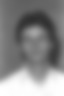
\includegraphics[width=0.2\textwidth]{blur_03_in} &
            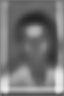
\includegraphics[width=0.2\textwidth]{blur_03_ep_1} &
            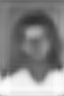
\includegraphics[width=0.2\textwidth]{blur_03_ep_5} &
            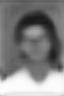
\includegraphics[width=0.2\textwidth]{blur_03_ep_10} &
            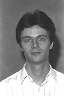
\includegraphics[width=0.2\textwidth]{96_64_target} \\
        \hline
            
\includegraphics[width=0.2\textwidth]{mosaic_05_in} &
            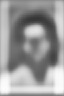
\includegraphics[width=0.2\textwidth]{mosaic_05_ep_1} &
            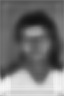
\includegraphics[width=0.2\textwidth]{mosaic_05_ep_5} &
            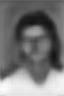
\includegraphics[width=0.2\textwidth]{mosaic_05_ep_10} &
            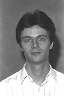
\includegraphics[width=0.2\textwidth]{96_64_target} \\
        \end{tabular}
    \end{adjustwidth}
\end{figure}

\clearpage
